\chapter{Preliminaries}
\label{chapter:preliminaries}
This chapter introduces metalearning -- learning how to learn. We begin with defining instances of data called datasets using a relation theory. We also discuss possible domains of relations and establish some restrictions for the rest of the thesis. The space of datasets is defined. We elaborate on specific problems that are connected with defining a structure on this space. Machine learning tasks are introduced and divided into three basic types -- \emph{supervised}, \emph{unsupervised} and \emph{reinforcement learning} -- based on the amount of feedback received from the environment. Then, we discuss the means to evaluate the performance of machine learning algorithms over machine learning tasks, namely \emph{root mean squared error}, \emph{F-measure} and \emph{predictive accuracy}. We discuss the existence of algorithm outperforming all other algorithms. We elaborate on the No Free Lunch theorem \cite{NoFreeLunchTheorem} and its implication on the machine learning tasks. The work of Smith-Miles et al. is reviewed \cite{SmithMilesTowardsMeasuresOfAlgorithmPerformance} as an interesting example of finding algorithms dominating a subset of data. We define the task of metalearning and we provide several examples of it -- dynamic parameter adjustment, and recommending machine learning algorithms for a given -- not yet seen -- task. The different algorithm recommendation are analysed, depending on the amount of information one requires from recommendation techniques - single algorithm, subset of them, more detailed ranking or even estimating the performance of algorithms. We discuss how generic methods for algorithm ranking should look like and define distance based ranking. We also review some of the related literature including our own results with hierarchical clustering \cite{jaICMLA2013}. Means of measuring the quality of a ranking are provided. The very simple and often effective baseline algorithm for the ranking task is introduced. The different types of performance indicators are reviewed together with some interesting approaches how to combine accuracy and time. Different types of metadata are defined. State of the art means of utilizing such metadata for the sake of algorithm recommendation are reviewed. We introduce a concept of automated systems able to handle the whole task of metalearning. Our own recommendation system Pikater is reviewed. We discuss PCA \cite{pca} method that can be used for visualization of multi-dimensional data.

\section{Datasets}
\label{section:datasets}
Dataset describes the instance of data. It can be a relation, set of graphs, collection of texts or database of proteins. Throughout this thesis, unless mentioned otherwise, we will consider the dataset to be of a form of relation \cite{dbRelation}.

\begin{definition}
	\emph{Relation} is a set of tuples $(d_1, \dots, d_n)$, where each element $d_j$ is a member of $D_j$, a data domain or data type.
\end{definition}

Given the relation, the dataset itself has a structure in the sense that every row is a vector of the same size and from the domain given by $D_1, \dots , D_n$. Alternatively, one can look at a dataset as a list of columns where every column has a domain and a collection of values. Sizes of all collections are the same.

We will specify three basic allowed supertypes:
\begin{enumerate}
	\item \emph{Categorical} supertype - domain is a finite set of values sometimes referred to as labels.
	\item \emph{Numerical} supertype - domains are real numbers -- $\mathbb{R}$.
	\item \emph{Integer} supertype - domains are integer numbers -- $\mathbb{N}$.
\end{enumerate}
Based on these supertypes, we will put domain restrictions on datasets that will be considered in this thesis. Every domain must be one of the defined supertype, possibly equal to the supertype or with some other restrictions (e.g. specified minimum, maximum). In this sense, the numerical supertype is also a supertype of the integer supertype. We have decided to distinguish this special case, as additional useful properties may be defined for the integer supertype only. We will also allow for some values to be undefined (missing).

We will define \emph{dataset space} as the space of all possible datasets. It is important to consider that now the dataset space is merely a set
without any added structure. Although every dataset has a structure defined by the relation, one cannot easily follow this when proposing a structure on the dataset space for the following reasons:
\begin{itemize}
	\item Number of columns may differ: the arity of relations representing datasets may vary. 
	\item Domains may differ: domains of columns may be different.
	\item Number of rows may differ: the cardinality of relations may differ.
\end{itemize}
Adding the structure into the dataset space is one of the main topics in the rest of the thesis.
\section{Machine Learning Tasks}
\label{section:mlTasks}
\emph{Machine learning} is a subfield of computer science. We say that algorithm is learning if it improves its performance on future tasks after making observations (receiving feedback) about the world \cite{aima3ed}.
According to the type of feedback, we can distinguish three main types of machine learning tasks.
\begin{definition}
	In \emph{unsupervised learning}, no explicit feedback is provided.
\end{definition}
A common unsupervised learning task is \emph{clustering}, when we try to sort input data to potentially interesting clusters. For example, an algorithm can eventually develop a concept of sunny and rainy days without ever being told this distinction.

On the opposite side stands the task of supervised learning, when we provide a teacher knowing the correct answers. Given a dataset, set of columns (usually only one) is designated as a target. 
\begin{definition}
	The task of \emph{supervised learning} is this: \\
	Given a \emph{training set} of $n$ example input-output pairs (rows of dataset)
	\begin{equation*}
	(x_1,y_1),\dots (x_n,y_n),
	\end{equation*}
	where $y_i$ is a vector of values of target columns of row $i$, $x_i$ is a vector of values of the remaining columns, each $y_i$ was generated by an unknown function $y=f(x)$, 
	discover a function $h$ that approximates the \emph{true function} f.
\end{definition}
 The function $h$ is called \emph{hypothesis}. The goal of learning is to search space of possible hypotheses finding the one that performs well, even on new examples beyond the training set. Note that in more general case, the input-output pair $x$ and $y$ do not have to be numbers or vectors, they can be labels, graphs or even more complex objects.

If the target attribute is only a single column, basic types of supervised learning can be defined by distinguishing the tasks according to the domain of target column $y$ -- classification or regression. 
In classification, we are assigning some labels to the input $x$. For example, when forecasting tomorrow's weather based on today's lookout, we could assign either sunny, cloudy or rainy.
\begin{definition}
	\emph{Classification} is a supervised learning task where the output y is one of the finite set of values. If the cardinality of the set is 2, we say it is a \emph{binary} or \emph{boolean} classification.
\end{definition}
On the other hand, in regression we are estimating some numeric value like tomorrow's temperature given today outlook.
\begin{definition}
	\emph{Regression} is a supervised learning task where the output y is a real number.
\end{definition}

To measure the quality of some hypothesis, the \emph{testing set} of previously unseen examples is given to the hypothesis. We say that $h$ \emph{generalizes} well if it correctly predicts the value $y$ for novel examples in the testing set. Sometimes, the learning algorithm exhibits low error on the training set while having poor generalization abilities. This phenomenon is called as \emph{overfitting} as the algorithm learned properties that are only specific for the training set. Usually, the algorithm capable of creating complex models tend to overfit on the simple data. To tackle this, the concept of \emph{ Occam's razor} is often used. If we have two hypothesis having similar performance, we should prefer the model with the lower complexity \cite{aima3ed}.

There are many ways of how to measure the quality of the hypothesis. We will list a few:

\begin{definition}
	\emph{Root mean squared error} (RMSE) of some hypothesis $h$ is defined as 
	\begin{equation*}
	RMSE(h)=\sqrt{\sum_{i=1}^{n}\frac{(h(x_i)-f(x_i))^2}{n}},
	\end{equation*}
	where $n$ is the number of samples in the testing set.
\end{definition}


In the binary classification we can define precision and recall:
\begin{definition}
	\emph{Precision} and \emph{recall} are defined as
	\begin{equation*}
	precision = \frac{tp}{tp+fp},
	\end{equation*}
	\begin{equation*}
	recall = \frac{tp}{tp+fn},
	\end{equation*}
	where $tp$ stands for true positive -- number of cases the classifier answered 1 correctly. Analogically, we can define $fp$ and $fn$ -- false positives and false negatives. They denote number of cases when classifier incorrectly answered 1 or 0 respectively.
\end{definition}
The common way to measure the quality of binary classifier is F-measure -- the harmonic mean of precision and recall.
\begin{definition}
	\emph{F-measure} of the hypothesis is
	\begin{equation*}
	F(h)=2\frac{precision\times recall}{precision+recall}.
	\end{equation*}
\end{definition}

In classification tasks, we can define the percentage of classes that were classified correctly or incorrectly resulting into the Predictive Accuracy and Error Rate. 

\begin{definition}
	\label{definition:predictiveAccuracy}
	\emph{Predictive Accuracy} is defined as
	\begin{equation*}
	PredictiveAccuracy = \frac{\#(h(x_i)=f(x_i))}{n},
	\end{equation*}
	where $n$ is the number of samples in the testing set.
	\emph{Error Rate} is defined as 
	\begin{equation*}
	ErrorRate = 1 - PredictiveAccuracy = \frac{\#(h(x_i)\ne f(x_i))}{n},
	\end{equation*}
	where $h$ is the hypothesis, $f$ is the true function, $n$ is the number of samples and $\#$ denotes the number of cases for which the argument is True.
\end{definition}

In the real world scenario, the reward is not often associated with every action. We often get a reward (or punishment) after a series of decisions. For example, if somebody wants to get from one place A to another place B, with every step taken he does not know whether the step was right. He can evaluate his decisions after he successfully gets to place B for example based on the time, money and energy needed to get to the destination. This concept is formalized as a third learning scenario -- reinforcement learning:
\begin{definition}
	The basic \emph{reinforcement learning} model consists of:
	\begin{enumerate}
		\item A set of environment states S.
		\item A set of actions A.
		\item Rules of transitioning between states.
		\item Rules that determine the scalar immediate reward of a transition.
		\item Rules that describe what the agent observes.
	\end{enumerate}
\end{definition}

\section{Metalearning}
This section describes the task of metalearning. Intuitively, it is a task of learning how to learn. We will discuss the metalearning task in general and then move to one particular subset of metalearning tasks -- algorithm recommendation. We will create a taxonomy of recommendation based on properties we would like to recommend.

\subsection{Metalearning Task}
In the recent years, many algorithms were proposed to solve different machine learning tasks. Usually, every such algorithm has many parameters and its performance is heavily dependent on settings of those parameters. Even for an expert, it is sometimes difficult to choose the right algorithm and set up the parameters correctly. Furthermore, scientists from different fields than computer science face great challenges when trying to employ machine learning to solve their tasks. It would be useful if such a system was provided that would either solve the machine learning tasks directly or would assist in choosing the right algorithms and parameters. Such a tool should learn from a previous experience. The common idea behind such recommendation tool is based on the idea that algorithms perform similarly on similar datasets.

One could also improve based on the past experience in adjusting the parameters. For example, if one non-deterministic machine learning experiment did not achieve desired performance for hundreds of attempts with the same parameter settings, it could be perhaps a good idea to try different settings next time. Also, if some indicators would suggest that the algorithm was being stuck in some local optimum, the parameters of the algorithm could be adjusted ad hoc, so the local optima are avoided and algorithm hopefully converges to a global optimum. The authors of \cite{algorithmControl} review the dynamic control of parameters for many nature inspired algorithms.

In transfer learning, we try to transfer some learned properties to a new -- similar -- task. For example, authors of \cite{TransferabilityDeepNeuralNetworks} argue that deep neural networks often learn a generally useful concept in the top layers and that such knowledge can be transferred to other tasks. The ability to transfer knowledge depends on the similarity of tasks.

These scenarios have some common patterns. In each case above, we are utilizing some extra knowledge -- previous experience or notion of dataset similarity -- usually referred to as \emph{metaknowledge}. This continuous process of learning how to learn is often denoted as metalearning.
In \cite{BrazdilMetalearning-2009}, we can find more formal definition of metalearning:
\begin{definition}
	\emph{Metalearning} is the study of principled methods that exploit metaknowledge to obtain efficient models and solutions by adapting machine learning and data mining processes.
\end{definition}

In this thesis, we will focus on the first case -- the \emph{algorithm selection} -- in which we use metaknowledge to recommend the best algorithms, parameters or both to some machine learning task. The problem was originally stated in 1976 by Rice \cite{1976RiceAlgorithmSelectionProblem} and received much attention from the research community ever since. Rice devised a general framework to select the best algorithm for a problem at hand. He suggested to extract set of \emph{metafeatures} out of a given problem and use these metafeatures to select an algorithm that maximizes the expected performance of the algorithm on the problem at hand.

One could naturally ask whether such recommendation is needed in the first place. Perhaps there exists an algorithm that is outperforming every other algorithm on every task. The answer is no. According to the \emph{No Free Lunch} theorem stated in \cite{NoFreeLunchTheorem}, the average performances of data mining algorithms on all data mining problems are equal. It can still be the case that there are some areas that are dominated by certain algorithms.

For instance, in \cite{SmithMilesTowardsMeasuresOfAlgorithmPerformance}, Smith-Miles et al. investigated different instances of optimization problems and features describing differences between these instances. The PCA (see Section \ref{section:pca}) was used to map features into two dimensional space.
Another instances were generated so the projected two dimensional space was better covered. The search algorithms were employed to find instances that are hard for each solver and provided a map of search space based on the expected footsteps of different optimization algorithms. The projected space of instances were coloured
according to colour of the dominating optimization technique on that space. This gave a nice overview of which part of two dimensional space computed by the PCA algorithm was dominated by which optimisation algorithm. This can be seen in Figure \ref{fig:smithMilesDominatedSpace}.

\begin{figure}
	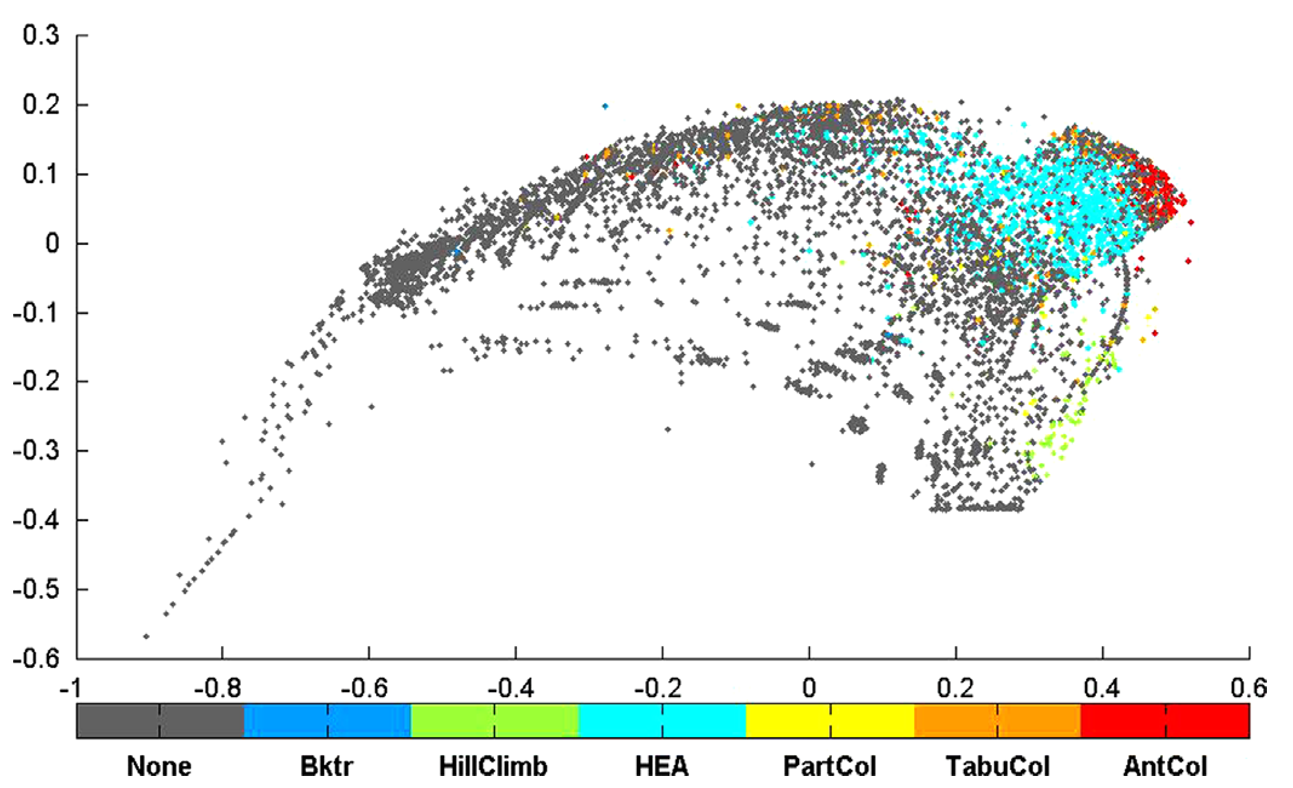
\includegraphics[width=14cm]{Images/smithMilesDominatedSpace.png}
	\centering
	\caption{Space of optimisation problems was projected to two dimensions by the PCA algorithm and coloured according to the best algorithm in that area. Grey colour is for the instances that had multiple best algorithms (according to some small margin) \cite{SmithMilesTowardsMeasuresOfAlgorithmPerformance}.}
	\label{fig:smithMilesDominatedSpace}	
\end{figure}


Another way to look at the No Free Lunch theorem is the fact that lots of problems from the set of all data mining problems may not be particularly interesting. One could argue that only problems related to some useful problem are worth considering. This argument is supported by the observation that usually when one learns something, he expects that the function being learned has some nice properties. For instance, it is continuous and close points have the same or similar value. For example, a car does not stop being a car if it changes a colour. One would have to make multiple adjustments to destroy the car properties. This arguing gives the notion to vaguely defined \emph{real world} problems. It follows that one should not be too concerned about the No Free Lunch theorem as it may still be the case that there is an algorithm outperforming every other algorithms on the real world problems.

In the rest of the thesis, we will solely focus on the algorithm selection problem.

\subsection{Types of Recommendation}
We can distinguish different types of algorithm selection \cite{BrazdilMetalearning-2009} based on what exactly we want to predict -- the \emph{metatarget}:
\begin{enumerate}
	\item Best in set.
	\item Best subset.
	\item Ranking.
	\item Performance prediction.
\end{enumerate}

The simplest case is choosing the best algorithm among the set of algorithms. This case has the advantage that it can be formulated as a classification problem. The major disadvantage is that if this algorithm produces unsatisfactory result, the recommendation system does not clue any steps to take further on. One may also choose to predict the best parameter for a certain algorithm.

More complicated case is when one is interested in some smaller subset of algorithms or parameters. The algorithms selected are those performing well -- this is often described as performing well within a margin. In the case of classification, the margin can be defined as 
\begin{equation}
\left[ e_{min}, e_{min}+k\sqrt{\frac{e_{min}(1-e_{min})}{n}} \right),
\end{equation}
where $e_{min}$ is the error of the best algorithm, $n$ is the number of examples and $k$ is a user-defined parameter determining the size of the margin.

Other alternative it to carry out statistical testing. The selected algorithms  will be those with not significantly worse performance than the best. Best subset address some flaws of the first type, however user does not have any guidance with the order of algorithms to try. Similarly, there is no guidance if all algorithms from the subset were tried.

In ranking, the goal is to rank (sort) algorithms or parameters according to their expected performance. In this case the exact performance value is not important, one is simply interested in the rank itself. One would naturally expect complete total ordering between algorithms or parameters. This does not have to be the case, sometimes this level of granularity is not desirable. For instance, one can decide that the algorithms with the similar expected performance will be inserted to a certain class and define the ordering just between the different classes of algorithms. The ordering between the algorithms of the same class could remain undefined. 

Based on these, we can distinguish different types of ranking based on the level of granularity provided. We can recognize linear and weak rankings (whether ranking defines linear order on some set of algorithms) and complete and incomplete rankings (whether rankings include all algorithms or just a subset). Rankings can be represented by \emph{Hasse diagrams} -- examples are in Figure \ref{fig:rankingTypes}.

\begin{figure}
	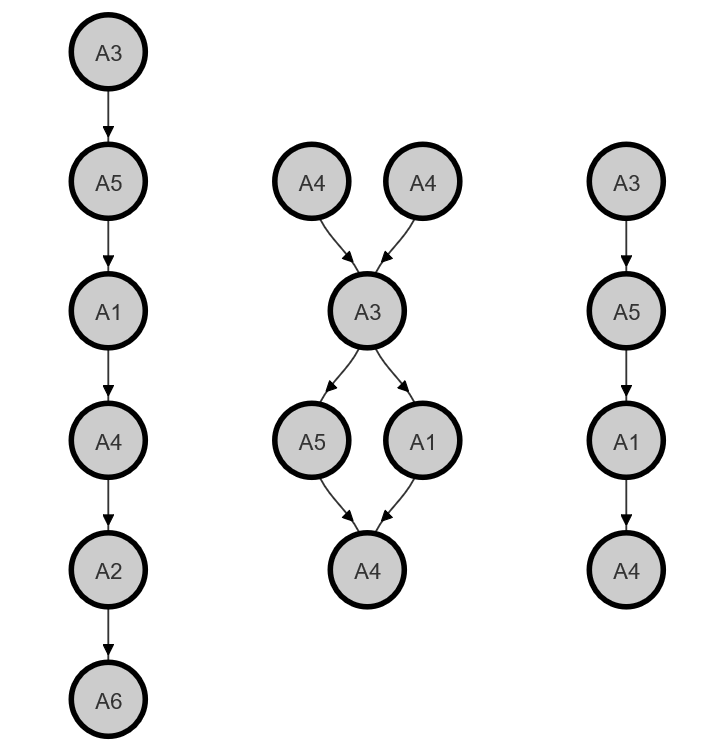
\includegraphics[width=8cm]{Images/rankingTypes.png}
	\centering
	\caption{Types of ranking. The left one is linear complete, middle one is weak and complete and the ranking on the right is linear and incomplete. Adapted from \cite{BrazdilMetalearning-2009}.}
	\label{fig:rankingTypes}	
\end{figure}

In some cases, one is not only interested in the ranking, but also in the performance estimation. This can be useful if there are some requirements for the minimal performance acceptable or if more detailed information about the expected outcome are required. It also makes sense if the estimated performance is the runtime of algorithm, as resources could be either limited or expensive, and algorithms that are expected to finish quickly are preferred. One could also expect that faster algorithms produce simpler hypothesis, thus arguing that on simple problems faster algorithms will have better generalization abilities by Occam's razor. 
The performance estimations can be easily transformed to ranking by ordering the algorithms by their estimated performance. 

Authors of \cite{evolutionaryProgramPredictingPerformance} propose a practical model of \emph{Evolutionary Program-induction Algorithms} (EPAs) including Genetic Programming (Section \ref{section:geneticProgramming}). The model corresponds to the following equation:
\begin{equation}
P(t) \approx a_0 + \sum_{p \in S}a_pd(p,t),
\end{equation}
where $a_i$ are coefficients, $P(t)$ is a performance of an EPA on the target functionality $t$, $S$ is a subset of a program search space and $d$ is a function of similarity between the output of the EPA and the target functionality $t$. The paper deals with the issue of determining the suitable coefficients and the suitable subset of the search space. The model is tested on various tasks.

In \cite{diplomka, jaIcannga2013}, we have predicted accuracy and expected time consumption  for some algorithm on a new dataset using the data gathered by our recommender system Pikater (see Section \ref{section:recommenderSystems}). A unique non-propositional distance measure was used (see Algorithm \ref{algo:attributeAlignmentMasterThesis}). 
Estimation functions were evolved by Genetic Programming and were represented by two trees: one for estimating accuracy and another one for estimating time consumption. The GP algorithm included terminals representing distance and the performance result (either accuracy or duration depending on the tree being evolved) from one of the nearest dataset. Randomly initialized constant terminal specified which nearest dataset was used. The special terminal estimating complexity was proposed: 
\begin{equation}
complexity = \sum_{a_i}\sigma(a_i)\log(n_{rows}),
\end{equation}
where $n_{rows}$ measures number of rows in the datasets, $a_i$ is the $i$-th attribute and $\sigma(a_i)$ estimates the attribute complexity based on its type:
	\begin{equation}
	\sigma(a_i)=
	\begin{cases}
	1; \text{ if  } a_i \text{ is a boolean or categorical attribute}, \\
	2; \text{ if  } a_i \text{ is an integer attribute}, \\
	3; \text{ if  } a_i \text{ is a real attribute}.
	\end{cases}
	\end{equation}
We argued that continuous and numerical attributes are usually hard to process, hence the increased coefficient. This complexity terminal proved especially useful for estimating the time needed to conduct the experiment.
The example of an evolved recommendation tree is in Figure \ref{fig:masterThesisTree}.
The recommendation agent utilizing the evolved estimation trees was implemented into our custom metalearning system called Pikater (see Section \ref{section:recommenderSystems}).

\begin{figure}
	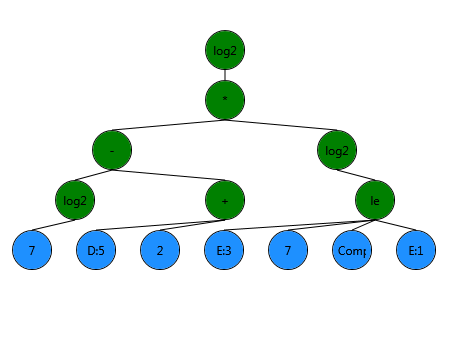
\includegraphics[width=14cm]{Images/masterThesisTree.png}
	\centering
	\caption{Example of the tree for estimating the algorithm duration on a new dataset. Terminals are blue, functions are green. The node labelled \emph{D:i} represents distance from the $i$-th nearest dataset. Similarly, the node labelled \emph{E:i} denotes error of the algorithm on the $i$-th nearest dataset. $Com$ is the complexity terminal. }
	\label{fig:masterThesisTree}	
\end{figure}

\section{Types of Metafeatures}
As devised in \cite{1976RiceAlgorithmSelectionProblem}, the extraction of metafeatures out of the problem at hand is needed for the algorithm selection problem. There are two main requirements for the metafeatures to extract -- the efficiency of the extraction and the descriptive factor of the metafeatures. The efficiency requirement is clear. The exact performance of all algorithms could be extracted as a feature but that would not give us any time savings at all. The question is what is an acceptable complexity. For instance, article \cite{metafeaturesNlogn} even suggests to restrict the complexity to $\mathcal{O}(n\log n)$ as bigger complexities are too expensive and it would be better to devote the time saved to already running some algorithms. We argue that the exact value depends on the algorithms in portfolio. With lots of algorithms and increased complexity of algorithms in portfolio, it still makes sense to compute even more expensive metafeatures. For example, if the portfolio contains NP-Complete problems, it should not be of concern to compute polynomial metafeatures. Furthermore, the suggestion is from the year 2000 and the significant increase of the CPU power and the ability to get more computational power instantly by using virtual servers in the cloud calls for not being so strict in limiting the complexity of computing the metafeatures. 

The second requirement also makes sense, as it is important to use the metafeatures that somehow help to distinguish between different algorithms. The rest is just noise and should be ignored, as even the computation of such noise can be costly.

We can distinguish metafeatures according to the nature of their computation.

The first category builds on statistic and information theory. Article \cite{MethodsForComparisonHenery1994} distinguishes three subcategories of the first category: \emph{simple}, \emph{statistical} and \emph{information-theoretic} measures. The simple measures include only very basic ones, such as the number of rows, the number of attributes or the number of integer attributes. 
Among the statistical ones, the article ranks such metafeatures as skewness, correlation, and kurtosis.
 Information-theoretic measures are motivated by information theory and are mostly appropriate for discrete attributes. The example of information-theoretic feature is \emph{entropy} of a discrete random variable: 
 \begin{equation}
 \label{equation:entropy}
H(X) = - \sum_{i}q_i\log_{2}q_i,
 \end{equation}
where $q_i$ is the probability that a variable $X$ takes on the $i$-th value. Conventionally, the entropy is converted to $\log_{2}$ as the measured value is in bits.

Authors of \cite{BrazdilMetalearning-2009} recognize two additional types of metadata -- \emph{model-based} and \emph{landmarkers}. The model-based metafeatures lies in training some sort of model on the data and take some properties of the model as metafeatures. For example, the decision tree \cite{decisionTrees} predicting the target is built. The number of nodes in the tree is introduces as a new metafeature. The landmarkers are a quick estimate of algorithm performance on the dataset. There are two ways how to do this. Either a simplified version of some algorithm is used to build the model on the whole data. For instance, the decision tree only with the top node is created and its performance evaluated on the data. Alternatively, \emph{subsampling landmarkers} use the whole algorithm on the subset of the data, which gives again the estimate.

From now on, we will treat dataset, unless stated otherwise, as the entity described by its metafeatures. We will distinguish two types of metafeatures. Propositional metafeatures (fixed size vector of metafeatures describing dataset as a whole) will be referred to in this thesis as \emph{global metafeatures}. The second type we will recognize are \emph{attribute metafeatures} -- that is the set of metafeatures extracted for each attribute in the dataset. As the number of attributes can vary per dataset, attribute metafeatures are non-propositional as we will have a vector of variable length of vectors of metafeatures. The vector of metafeatures does not have to be necessarily of a fixed size. Different types of attributes can have different types of metafeatures. We will address this in the later chapters.
The set of metafeatures will be also called metadata throughout the thesis. It can be argued that reshuffling the attributes of the datasets does not change the dataset at all. Therefore, we will consider two datasets represented by their metadata equal if and only if:
\begin{enumerate}
	\item All available global metadata are equal.
	\item All available attribute metadata are equal, or there exists a permutation (reshuffling) of attributes of the first dataset such that attribute metadata are equal after the reshuffling.
\end{enumerate}

\section{Distance Based Ranking}
\label{section:distanceBasedRanking}
In the previous sections, we have discussed the problem of algorithm ranking. The usual approach to the ranking is based on the idea that algorithms perform similarly on similar datasets. If we want to exploit this idea, we need two things -- a notion of distance between datasets and a way of calculating a ranking from the previous results on datasets similar to a dataset at hand using the distance between datasets.
In this section, we will focus on the latter and suppose that we already have the notion of distance. Throughout this thesis, when outlying the pseudocode of some algorithm, we will treat dataset distance measure as an interface taking two datasets and outputting a real number -- the measured distance between the both input datasets. This is formalized in Algorithm \ref{interface:IDatasetDistance}.

\IncMargin{1em}
\begin{algorithm}
	\SetKwData{Return}{return}
	\SetKwInOut{Input}{input}
	\SetKwInOut{Output}{output}
	\tcp{Interface for measuring distance between two datasets.}
	\Input{$a \leftarrow$ First dataset}
	\Input{$b \leftarrow$ Second dataset}
	\Output{ $d \in \mathbb{R}, d$ is a distance between $a, b$ $(d = \globalDistance(a,b))$ }
	\BlankLine
	\caption{$IDatasetDistance$: dataset distance interface}\label{interface:IDatasetDistance}
\end{algorithm}\DecMargin{1em}

This will enable us to plug different algorithms as the part of others. We will see lots of algorithms conforming to the $IDatasetDistance$ interface throughout the thesis. To avoid confusion, we will always use the symbol $\globalDistance$ when referring to the $IDatasetDistance$ interface in equations or other algorithms.

To allow for obtaining the ranking, we will define another interface called $IRanking$ -- the one that just takes a dataset and returns the ranking of algorithms to the given dataset. The interface is intentionally very generic, so we can reuse it later even with the non-distance based ranking. 

\IncMargin{1em}
\begin{algorithm}
	\SetKwData{Return}{return}
	\SetKwInOut{Input}{input}
	\SetKwInOut{Output}{output}
	\tcp{Interface for calculating the ranking to a new dataset.}
	\Input{$d \leftarrow$ dataset to rank}
	\Output{Ranking -- ordering of algorithms}
	\BlankLine
	\caption{$IRanking$: Interface for ranking calculation}\label{interface:IRanking}
\end{algorithm}\DecMargin{1em}

One could wonder how to implement $IRanking$ interface using distance based ranking. The $IRanking$ interface provides just a dataset on the input. But for the distance based ranking, at least the distance measure and other datasets need to be provided. 

To solve this, we will use a concept from functional programming.
\emph{Functional programming} \cite{functionalThinking} is a programming paradigm -- a style of building the structure and elements of computer programs -- that treats computation as the evaluation of mathematical functions. In this thesis, we will be proposing generic layered architecture of algorithms. As we want to design generic interface but the subcomponents will be initialized and parametrized differently, we will use specific functional programming construct know as partial application.

\begin{definition}
	\emph{Partial application} refers to the process of fixing a number of arguments to a function, producing another function of smaller arity. Given an integer $k$ and a function $f:X_1 \times \dots \times X_k \times \dots \times X_n \rightarrow Y$, the function $partial_k$  is defined as a function $X_1 \times \dots \times X_k \rightarrow (X_{k+1} \times \dots \times X_n \rightarrow Y)$. The $k$ is often omitted as it can be inferred from the number of input arguments.
\end{definition}

This will enable us to preinitialise some parameters and the remaining not yet assigned parameters will define the generic interface.

Because of the $partial$ application, we have an elegant way to solve the issue. We can define an interface taking all the necessary information to build up the distance based ranking and then just use $partial$ application to fix all the arguments except the dataset one. The resulting function now conforms to the $IRanking$ interface.
More formally, the $IDistanceRanking$ interface is defined in Algorithm \ref{interface:IDistanceRanking}.

\IncMargin{1em}
\begin{algorithm}
	\SetKwData{Return}{return}
	\SetKwInOut{Input}{input}
	\SetKwInOut{Output}{output}
	\tcp{Interface for calculating the ranking to a new dataset based on distance.}
		\Input{$\globalDistance \leftarrow IDatasetDistance$ - Dataset distance measure}
		\Input{exp $\leftarrow$ Previous results}
		\Input{$d \leftarrow$ Dataset to obtain ranking for}
		\Output{ Ranking -- ordering of algorithms }
	\BlankLine
	\caption{$IDistanceRanking$: Interface for distance based ranking calculation}
	\label{interface:IDistanceRanking}
\end{algorithm}\DecMargin{1em}

And the transformation of $IDistanceRanking$ interface to a more generic $IRanking$ interface is outlined in Algorithm \ref{algorithm:IDatasetRankingTransformarmation}.
\IncMargin{1em}
\begin{algorithm}
	\SetKwInOut{Input}{input}
	\SetKwInOut{Output}{output}
	\tcp{Interface for transforming $IDistanceRanking$ to $IRanking$.}
	\Input{distanceRanking $\leftarrow IDistanceRanking$ interface}
	\Input{$\globalDistance \leftarrow IDatasetDistance$ - Dataset distance measure}
	\Input{exp $\leftarrow$ Previous results}
	\Output{$IRanking$ interface}
	\BlankLine
	\Return partial(distanceRanking, $\globalDistance$, exp)\;
	\caption{Distance Ranking Transformation: transforming a $IDistanceRanking$ interface to generic $IRanking$ interface}
	\label{algorithm:IDatasetRankingTransformarmation}
\end{algorithm}\DecMargin{1em}

Now we can propose several algorithms that can be implemented to conform to the $IDistanceRanking$ interface.

The \emph{$k$-Nearest Neighbours} algorithm ($k$-NN) \cite{knn} is widely used for ranking~\cite{BrazdilMetalearning-2009}. For instance, Maratea et al. use $k$-NN in their system for solving \emph{answer set programming task} (ASP) \cite{MarateaMEASPProgressReport,MarateaMeAsp}. ASP is a declarative approach towards hard (mainly NP) search problems. The $k$-NN algorithm for ranking is aggregating previous results on the $k$ nearest neighbours identified by the distance measure to estimate the ranking. The whole method is outlined in Algorithm \ref{algo:k-nnRanking}. The complexity, provided that a distance is already precomputed, is $\mathcal{O}(n_d\log(n_d)+n_a\log(n_a))$, where $n_a$ is the number of algorithms and $n_d$ the number of datasets. If the ranking is called multiple times for different datasets, the computation of the distance could be repeated, therefore it is often useful to compute the distance outside of this function. This was the reason why we stated the complexity for already precomputed distance. This will be our case as we need lots of ranking computation to evaluate the quality of ranking algorithm. This is mainly a technicality, so for the sake of simplicity, we will not state explicitly in the algorithms that we are computing something outside of the algorithm when plugging the algorithms into one another. 

\IncMargin{1em}
\begin{algorithm}
	\SetKwInOut{Input}{input}
	\SetKwInOut{Output}{output}
	\tcp{Implementation of $IDistanceRanking$ using $k$-NN algorithm}
		\Input{$k \leftarrow$ Number of neighbours}
		\Input{$\globalDistance \leftarrow IDatasetDistance$ Dataset distance measure}
		\Input{exp $\leftarrow$ Previous results}
		\Input{$d$ $\leftarrow$ Dataset to obtain ranking for}
		\Output{ Ranking }
	\BlankLine	
	distances $\leftarrow []$\;
		\ForEach{\upshape dataset $\in$ exp.datasets}{
			current\_distance $\leftarrow \globalDistance(d,\text{ dataset})$\;
			distances $\mathrel{+}=  [(\text{dataset, current\_distance})]$\;
		}
		distances $\leftarrow$ sort(distances, (dataset, distance):distance)\;
		neighbours $\leftarrow$ distances$[:k]$\;
		\ForEach{\upshape algorithm $\in$ exp.algorithms}{			
				$r_{\text{algorithm}} \leftarrow 0$\;
		}
		\ForEach{\upshape neighbour $\in$ neighbours}{
					\ForEach{\upshape algorithm $\in$ exp.algorithms}{			
				$r_{\text{algorithm}} \mathrel{+}=$ exp.rank(neighbour, algorithms)\;
			}
		}		
	$R \leftarrow [1, \dots$ len(exp.algorithms)$]$\;
	$R \leftarrow$ sort($R$, algorithm: $r_{\text{algorithm}}$)\;
	\Return $R$\;
	\caption{$K$-NN Ranking: $k$-NN based implementation of $IRanking$.}
	\label{algo:k-nnRanking}
\end{algorithm}\DecMargin{1em}

The $k$-NN algorithm can be also modified in such a way to involve the weights into computation, so that closer neighbours have bigger influence on the final result \cite{weightedKnn}.
The number of neighbours -- $k$ -- is the crucial parameter of the whole algorithm. Setting of $k$ to 1 or similarly low values usually results in overfitting and corresponding bad generalization abilities of the model. On the other hand, high values of $k$ defeat the purpose of the local neighbourhood and tend to have lower performance as the information from the distant regions affect the decision process. To address this, there has been also some additional modifications proposed to the $k$-NN algorithm. The \emph{G-means} algorithm \cite{gmeans} enhances the original algorithm by automatically setting the number of neighbours. The G-means is based on a statistical test for the hypothesis that a subset of data follows a Gaussian distribution. The G-means runs $k$-means with increasing $k$ in a hierarchical fashion until the test accepts the hypothesis that the data assigned to each $k$-means centre are Gaussian. Two key advantages are that the hypothesis test does not limit the covariance of the data and does not compute a full covariance matrix. The $G$-means algorithm was used for algorithm selection by authors of \emph{Autofolio} \cite{FrankHutterAutomaticallyConfiguredAlgorithmSelector}. The G-means is used together with other algorithms for automatic selection of parameters to solve some artificial intelligence problem at hand (e.g. \emph{satisfiability} (SAT), \emph{constraint satisfaction programming} (CSP) or \emph{quantified boolean formula} (QBF)). In \cite{algorithmSelectionAndScheduling}, the G-means is used in algorithm portfolio selection of the SAT solvers. Motivated by the observation that solvers have complementary strengths and therefore exhibit incomparable behaviour on different problem instances, algorithm portfolios run multiple solvers in parallel or select one solver, based on the features of a given instance. 

In \cite{jaICMLA2013}, we investigated the possibility of distance based ranking using clustering constructed from the training set. In our case, the clustering  was a result of an \emph{agglomerative clustering algorithm} \cite{hierarchicalClustering}. The advantage of this clustering method is that it does not require creation of centroids as in the case of other methods. Compared to the $k$-NN algorithm, the neighbourhood does not have a fixed size but rather a variable size depending on the cluster method.

The bottom up method was chosen because it is faster than the top down method. The question arises which criterion of clusters’ distance to use. We have adopted \emph{Unweighted Pair Group Method with Arithmetic Mean} (UPGMA), or average linkage clustering \cite{hierarchicalClustering}, which is used in various applications~\cite{hierarchicalClusteringApplications}.

In our experiments, ranking was constructed the same way as in the $k$-NN ranking algorithm with the exceptions that the nearest neighbours of the given dataset were selected according to the nearest cluster, given metric and UPGMA method. In the experiments, we have used the results of 8 \emph{Weka} \cite{weka} algorithms on the 85 \emph{UCI} (Dataset Repository of University of California, Irvine) \cite{uci} datasets. The datasets were divided into the training and testing set with the ratio of 2:1. We have tested various distance metric to estimate the algorithm performance. Results indicated that such hierarchical clustering can be successfully used for metalearning. The best dendrogram of the best cluster is shown in Figure~\ref{fig:dendrogram}. 

\begin{figure}
	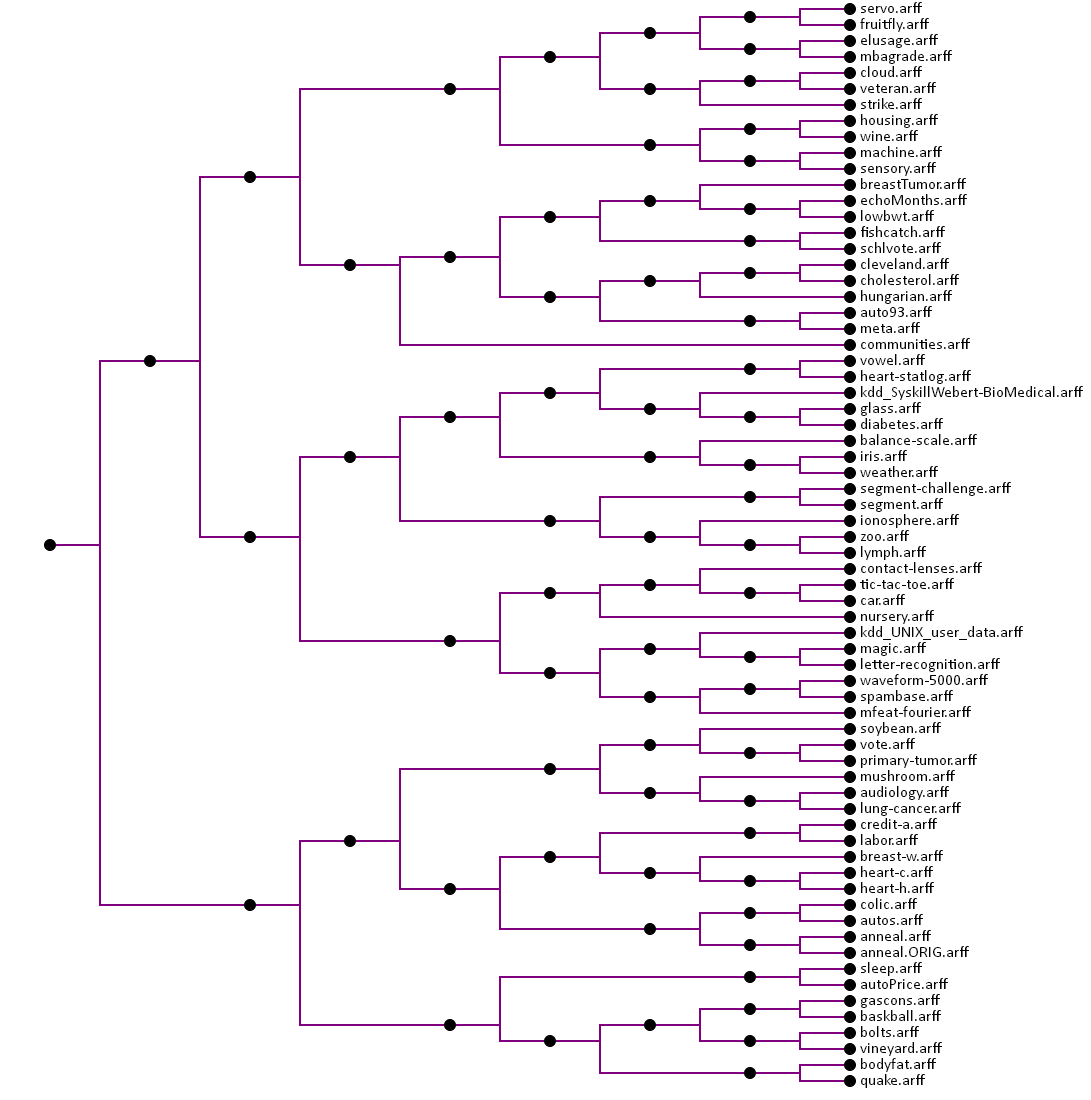
\includegraphics[width=14cm]{Images/tree.png}
	\centering
		\caption{The dendrogram as a result of the agglomerative clustering \cite{jaICMLA2013}. Datasets are assigned to clusters according to their similarity.}
		\label{fig:dendrogram}	
\end{figure} 
 
\section{Assessing the Ranking Quality}
\label{section:rankingQuality}
In this section, we describe techniques to asses the quality of some method for predicting the ranking of algorithms. 
Given some $IRanking$ interface implementation and a new dataset $d$, the \emph{Spearman's rank correlation coefficient} can be used to asses the accuracy of the ranking method:
\begin{equation}
\label{eq:spearman}
r_s^d=1-\frac{6\sum_{i=1}^{n}(R^{'d}_i-R^d_i)^2}{n^3-n},
\end{equation}
where $n$ is the number of models, $R^d_i$ is the actual rank of model $i$ on dataset $d$ and $R^{'d}_i$ is the predicted rank of model $i$ on dataset $d$. The Spearman's rank correlation coefficient has some interesting properties. The range of the coefficient is normalized to the interval $\langle-1,1\rangle$, where 1 is a perfect match, -1 is a perfect mismatch and 0 indicates results as good as random guessing.
Equation \ref{eq:spearman} gives us the means of measuring ranking quality for a single dataset. If the aim is to measure the quality over all datasets, it is possible to take Spearman's rank correlation coefficient averaged over all datasets: 
\begin{equation}
\label{eq:averageSpearman}
r_s=\frac{\sum_{d=1}^{n}r^d_s}{n},
\end{equation}
where $n$ is the number of datasets and $r^d_s$ is the Spearman's rank correlation coefficient computed for dataset $d$.

The whole ranking quality assessment is summarized in Algorithm \ref{algo:rankingQualityEvaluation}.
\IncMargin{1em}
\begin{algorithm}
	\SetKwInOut{Input}{input}\SetKwInOut{Output}{output}
	\tcp{Pseudocode for ranking prediction quality assessment using dataset distance function.}
	\Input{datasets $\leftarrow$ List of datasets}
	\Input{predictor $\leftarrow IRanking$ Ranking predictor}
	\Input{results $\leftarrow$ Results of algorithms on datasets indexed by datasets}
	\Input{algorithms $\leftarrow$ List of algorithms}
	\Output{Ranking Prediction Quality Assessment}
	\BlankLine
	$r_s\leftarrow$ 0\;
	$n \leftarrow$ len(algorithms)\;
	\ForEach{\upshape dataset $\in$ datasets}{
		remaining $\leftarrow$ datasets $\setminus$ dataset\;
		$R^{\text{dataset}} \leftarrow$ predictor(dataset, remaining, results, algorithms)\;		
		$r_s^{\text{dataset}} \leftarrow  1-\cfrac{6\sum_{i=1}^{n}(R^{\text{dataset}'}_i-R^{\text{dataset}}_i)^2}{n^3-n}$\;
		$r_s \leftarrow r_s+\cfrac{r_s^{\text{dataset}}}{n}$\;
	}
	\Return $r_s$\;
	\caption{Ranking Quality Assessment}\label{algo:rankingQualityEvaluation}
\end{algorithm}\DecMargin{1em}

Basically, the algorithm for each dataset estimates the ranking of algorithms by using $IRanking$ interface. The quality of rankings is measured using Equation \ref{eq:averageSpearman}. Provided the predictions are already precomputed, we get a complexity of the quality evaluation: $$\mathcal{O}(n_dn_a),$$
where $n_d$ is the number of datasets and $n_a$ is the number of algorithms.

\section{Ranking Baseline}
\label{section:baseline}
Algorithm \ref{algo:rankingQualityEvaluation} can give us a good estimate of how good our model is compared to random guessing. However, there may be trivial methods that are very easy to implement, yet they exhibit a relatively good performance. Such trivial algorithms are often referred to as \emph{baseline} algorithms. Their output is usually based on some statistical knowledge about the data and is calculated using the most frequent values. Complex algorithms should outperform baseline algorithms, otherwise there is no need for the extra complexity.
In the classification tasks, the baseline usually outputs the most frequent class. In the regression task, the median or average of the target values is usually returned by the baseline algorithm. We can also define a baseline algorithm for the ranking task. The baseline algorithm can predict the ranking results based on algorithm's average rank on all datasets present in the metaknowledge base. If one algorithm is the best in average on all datasets, baseline algorithm will just assign the first rank to this algorithm. Again, we will design the baseline algorithm with the $IRanking$ interface in mind. To calculate the ranking, baseline needs the information about the average ranking. One could be tempted to use again the trick with the $partial$ function. In this case this would be a mistake, as that would result in recalculating the average ranking for each call to the interface. Instead, we will create a function that takes previous results as an input, calculates average ranking, and then returns a function conforming to the $IRanking$ interface. Such course is outlined in Algorithm \ref{algo:rankingBaseline}. The complexity of resulting $IRanking$ is constant. To build up the distance, one has to do $$\mathcal{O}(n_dn_a + n_a\log(n_a))$$
steps, where $n_d$ is the number of datasets and $n_a$ is the number of algorithms. The term $(n_dn_a)$ represents the cost of two inner loops, the term $n_a\log(n_a)$ is for sorting the rankings.
\begin{algorithm}
	\SetKwInOut{Input}{input}
	\SetKwInOut{Output}{output}
	\tcp{Pseudocode for building the ranking baseline model.}
	\Input{datasets $\leftarrow$ List of datasets}
	\Input{algorithms $\leftarrow$ List of machine learning algorithms}
	\Input{results $\leftarrow$ Results of algorithms on datasets indexed by datasets}
	\Output{$IRanking$ interface}
	\BlankLine
	averageRanking $\leftarrow []$\;
	occurrences $\leftarrow []$\;
	\ForEach{\upshape algorithm $\in$ algorithms}{
		averageRanking[algorithm]$\leftarrow 0$\;
		occurrences[algorithm] $\leftarrow 0$\;
	} 
	\ForEach{\upshape dataset $\in$ datasets}{
		resultsOnDataset $\leftarrow$ results[dataset]\;
		\ForEach{\upshape algorithm $\in$ algorithms}{
			\If{\upshape algorithm $\in$ resultsOnDataset}
			{
				occurrences[algorithm]$\mathrel{+}\mathrel{+}$\;
				currentRank $\leftarrow \cfrac{\text{resultsOnDataset[algorithm]}}{\text{len(resultsOnDataset)}}$\;
				averageRanking[algorithm]$\mathrel{+}=$ currentRank\;
			}
		}
	}
	averageRankingWithAlgorithm $\leftarrow$ zip(averageRanking,algorithms)\;
	averageRankingWithAlgorithm $\leftarrow$ map(averageRankingWithAlgorithm,$\lambda(x,y)\rightarrow \cfrac{x}{occurrences[y]},y)$\;
	averageRankingWithAlgorithm$\leftarrow$ sort(averageRankingWithAlgorithm,$(x,y):x$)\;
	\Return $\lambda(x) \rightarrow $ averageRankingWithAlgorithm\;
	\caption{Ranking Baseline}\label{algo:rankingBaseline}
\end{algorithm}\DecMargin{1em}

\section{Performance Indicators}
In the previous sections, we have discussed the metatarget and ranking in particular. We did not discuss what should be the performance indicator defining the metatarget. It can be any of the performance measures mentioned in Section \ref{section:mlTasks} or a combination of them. The time complexity can also be predicted or time can be included into the performance consideration. This is useful when good and fast learning algorithms are preferred.  The time is especially crucial when the resources are scarce or expensive.

The time cost value of following some ranking strategy is captured by the \emph{top-$N$} evaluation \cite{topNEvaluation}. The $N$ is a parameter that determines how many best algorithms will be tried on some dataset. Different settings of $N$ can be consequently simulated, and we can observe how the accuracy of the best model improved compared to the time cost associated with the increase of $N$.

The top-$N$ strategy has a disadvantage that it is unable to leverage what is learned from previous evaluations.
Alternatively, we can tackle this issue with a strategy called \emph{active testing} \cite{activeTesting}. It proceeds in a tournament-style fashion, in each round selecting and testing the algorithm that is most likely to outperform the best algorithm of the previous round on the new dataset. The next contender is selected based on the concept of \emph{relative landmarkers} \cite{relativeLandmarkers}. These landmarkers estimate the relative probability that a particular algorithm will outperform the current best candidate. The \emph{cross-validation} \cite{aima3ed} of the new contender is performed. The result is added to the relative landmarkers and the contender replaces the current best algorithm if the cross-validation result is better or ties the result of current best algorithm.

One approach of combining time and accuracy was proposed by Brazdil et al. \cite{Brazdil00zoomedranking}. The $k$-Nearest Neighbours algorithm \cite{knn} with a distance function based on a set of statistical, information theoretic, and other dataset characterization measures is employed in order to identify the set of similar already computed tasks. For the ranking phase, the adjusted ratio of ratios ranking method is presented, which processes performance information based on accuracy and time.

The relevance of the processed dataset $d_i$ to the dataset $d_j$ at hand is defined in terms of similarity between them, according to metafeatures. It is given by a metric (or a distance function):
\begin{equation}
\globalDistance\left(d_i,d_j\right)=\sum_{x} \sigma\left(v_{x,d_i},v_{x,d_j} \right),
\end{equation}
where $d_{i}$ and $d_j$ are datasets, $v_{x,d_i}$ is the value of metafeature $x$ for dataset $d_i$, and $\sigma\left(v_{x,d_i},v_{x,d_j} \right)$ is the distance between the values of metafeature $x$ for datasets $d_{i}$ and $d_j$. All metafeatures are normalized.

The $k$-Nearest Neighbours algorithm is then used to identify the $k$ cases nearest to the dataset at hand.

The \emph{adjusted ratio of ratios} uses information about accuracy and execution time to rank the given classification algorithms. It is computed by means of the auxiliary term ${ARR}_{a_p,a_q}^{d_i}$ defined as:

\begin{equation}
{ARR}_{a_p,a_q}^{d_i}=\frac{\frac{SR_{a_p}^{d_i}}{SR_{a_q}^{d_i}}}{1+\frac{\log{\left(\frac{T_{a_p}^{d_i}}{T_{a_q}^{d_i}}\right)}}{K_T}},
\end{equation}
where $SR_{a_p}^{d_i}$ and $T_{a_p}^{d_i}$ are the success rate and duration of algorithm $a_p$ on the dataset $d_i$, and $K_T$ is a user-defined value that represents the amount of accuracy the user is willing to trade for a 10 times speed-up or slowdown. For example, $K_T$ = 10\% means that the user is willing to trade 10\% of accuracy for 10 times speed-up. 

Finally, the overall mean adjusted ratio of ratios for each algorithm is derived:
\begin{equation}
{ARR}_{a_p}=\frac{1}{m-1}\left(\sum\nolimits_{a_q} \frac{\sum\nolimits_{d_i} {{ARR}_{a_p,a_q}^{d_i}}}{n} \right),
\end{equation}
where $m$ is the number of algorithms and $n$ is the number of datasets. The ranking is based on this measure.
Authors of \cite{brazdilArrCorrected} including one of original authors of $ARR$ looks into the $ARR$ measure and argue that $ARR$ should be monotonically increasing Higher success rate ratios should lead to higher values of ARR and, similarly, higher time ratios should lead to lower values of ARR. Experiments were proposed to verify this property on data. The $\frac{SR_{a_p}^{d_i}}{SR_{a_q}^{d_i}}$ was fixed to 1, the time ratio was sampled from very small $2^{-20}$ to very high values $2^{20}$ and three different values of $K_T$ were used ($0.2, 0.3, 0.7$). The resulting ARR function was not monotonic and was even approaching infinity at some point. In general, this can lead to incorrect rankings provided by the metalearner and can affect the evaluation results. Authors proposed a solution that addresses this issue by changing the re-sampling used in $ARR$. The updated formula $A3R$ was proposed:
\begin{equation}
{A3R}_{a_p,a_q}^{d_i}=\frac{\frac{SR_{a_p}^{d_i}}{SR_{a_q}^{d_i}}}{\sqrt[n]{\frac{T_{a_p}^{d_i}}{T_{a_q}^{d_i}}}},
\end{equation}
where $n$ is a user defined constant representing the importance of time.

The $A3N$ is used in \cite{brazdil_a3rExperiments} as a performance indicator. The paper proposes several modification to active testing strategy \cite{activeTesting}. The first approach uses faster sample-based tests to identify competitive algorithms. The second modification lies in argument that full cross-validation test is not necessary to estimate the next candidate. Instead, the test is performed on a smaller sample of the new dataset. This is motivated by the fact that a sample-based test is much faster than a full cross-validation test. The full cross-validation test is carried out only if a candidate algorithm beats the currently best algorithm on the sample-based test.

\section{Systems for Algorithm Recommendation}
\label{section:recommenderSystems}
Having a viable framework for metalearning is only one side of a coin. The actual systems built for metalearning are called \emph{recommendation system}. Their goal is to allow for a trade-off between human time and machine time. They can also provide the power of machine learning algorithms to the non-expert users, even to those with limited computer knowledge. There are many scenarios for such systems.

\emph{Auto-weka} \cite{autoWeka} is a system integrating into the Weka toolkit \cite{weka} and it is able to perform model selection, and autotune model parameters. It employs the \emph{Sequential Model-based Algorithm Configuration algorithm} (SMAC) \cite{autoWekaSMAC}. SMAC supports a variety of models of the type $p(c| \lambda)$ to capture the dependence of the loss function $c$ on hyper-parameters $\lambda$, including approximate Gaussian processes~\cite{gaussianProcesses} and random forests \cite{randomForests}. 

Autofolio \cite{FrankHutterAutomaticallyConfiguredAlgorithmSelector} combines SMAC with algorithm selection framework claspfolio2~\cite{claspfolio2}. \emph{Claspfolio2} is a flexible framework that provides functionality to train and assess the performance of different algorithm selection techniques. The extensibility is the main advantage and it provides an unified framework for algorithm selection problem. The overview of all components is in Figure \ref{fig:claspfolio2}. The scheduling system is also integrated.

\begin{figure}
	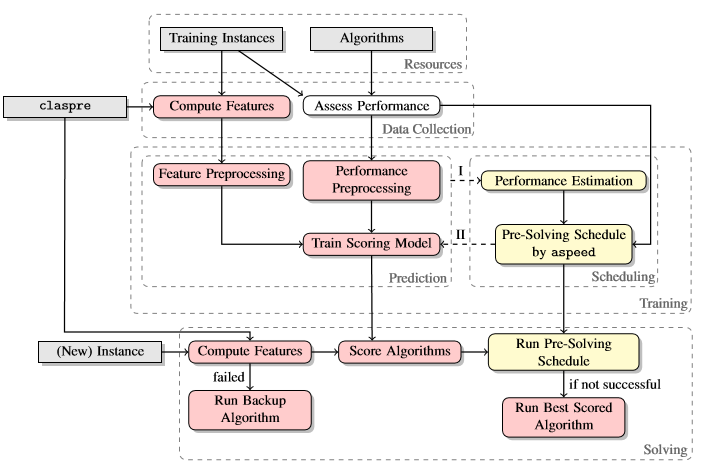
\includegraphics[width=14cm]{Images/claspfolioSchema.png}
	\centering
	\caption{Overview of claspfolio2 framework \cite{claspfolio2}.}
	\label{fig:claspfolio2}	
\end{figure}

Our recommendation system called \emph{Pikater} \cite{jaPikater, icmlaHawaii, wiat11, KazikIAENG} is implemented using \emph{multi-agent systems} (MAS). To be precise, the multi-agent framework \emph{JADE} \cite{JADE} is used as a platform of the system. The extensibility is assured by the use of the structured ontology language and following the \emph{Foundation for Intelligent Physical Agents} (FIPA) \cite{FIPA} international standards of agents' communication. The following basic scenarios have been considered.
\begin{itemize}
	\item In the most simple case, the user knows which method and what parameters of that method they would like to use.
	\item In the second scenario, the user knows what method to use but does not know how to set its parameters. The system is able to search the parameter space of the method and find a setting that provides good results. 
	\item In the third case, the user does not even know what method to use and lets the system decide by itself. In this case, the system recommends the best possible method or provides a ranking of the methods based on predicted errors and duration.
\end{itemize}
These simple scenarios can be extended into more complex ones. For instance, it is also possible to combine the recommendation of the best method with parameter space search, when the system recommends an interval of the parameter’s values. As a positive side effect, the metaknowledge base for metalearning purposes is being built up by each experiment. 

In order to effectively design our system, we have chosen the organization-centred formalism \emph{AGR} (Agent-Group-Role) \cite{agr}. The role is a set of capabilities and responsibilities that the agent accepts by handling the role. Group — the building block of a MAS — is a set of agents with allowed roles and interactions, defined by a group structure. The multi-agent system then consists of multiple groups which can overlap, as agents can belong to more than one group. In this formalism, we abstract from the algorithmic details and inner logic of the agents in the MAS. Authors of \cite{KazikIAENG} used the ontological formalism of \emph{OWL-DL} \cite{pelletOwlDl} to describe the organizational model of Pikater. The following group structures were defined according to the aforementioned scenarios: administrative group structure, computational group structure, search group structure, recommendation group structure, data group structure, and data-management group structure. Our MAS is composed of groups that are instances of these group structures. The architecture is depicted in Figure \ref{fig:pikaterArchitecture}.


\begin{figure}
	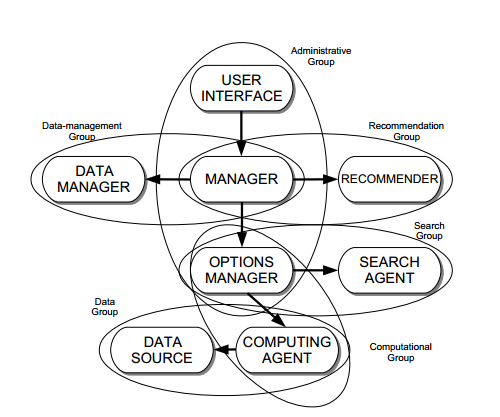
\includegraphics[width=14cm]{Images/pikaterArchitecture.png}
	\centering
	\caption{Overview of Agent-Group-Role model of our recommendation system Pikater \cite{jaPikater}.}
	\label{fig:pikaterArchitecture}	
\end{figure}

The MAS-based solution allows for a flexibility in choice of the parameter space search algorithms, each of these is encapsulated in a search agent. General tabulation, random search, simulated annealing \cite{aima3ed}, or parallel methods, such as genetic algorithms, are implemented in our system. Another great benefit of the agent-based approach is the natural capability to parallelly execute multiple computations with various parameters. This significantly decreases the time needed for the execution of the parameter space search process. One of essential features of our MAS is its capability of recommending a suitable computational method for a new dataset, according to datasets similarity and previously gathered experience. The choice of the similar dataset(s) is based on various previously proposed metrics \cite{hierarchicalClustering}, which measure the similarity of their metadata. Our database contains over 600,000 records, that are used to suggest the proper method (including its parameters) and estimate its performance on a new dataset. The latest version of our MAS contains the following types of recommenders, which differ in the metric used and in the number of recommended methods they provide:
\begin{itemize}
	\item Basic recommender chooses a method based on the single closest dataset using the unweighted metadata metric.
	\item Clustering Based Classification \cite{jaICMLA2013} chooses the whole cluster of similar datasets and the corresponding methods, using different sets of metadata features.
	\item Evolutionary Optimized Recommenders are similar to the two above described recommender types, using different weighted metrics, optimized by an evolutionary algorithm.
	\item Interval Recommender recommends intervals of suitable parameter values and leaves their fine-tuning to the parameter space search methods.
\end{itemize}
Another functionality of our system is a multi-objective optimization of data mining configurations. To test this, the search algorithm is employed in order to find beneficial combinations of pre-processing and machine learning methods to the presented data. The minimization is performed in error-rate as well as run-time criteria \cite{Kazik2015}.

\section{Related Work}
In this section, we further review some of the literature related to metalearning. Authors of \cite{KazikPesk} define the distance between datasets based on the following metadata:
\begin{itemize}
	\renewcommand{\labelitemi}{$\bullet$}
	\item \textit{Number of attributes} in data,
	\item \textit{Number of instances},
	\item \textit{Data type} (Relates to all values of all attributes in the dataset. Four categories of data are considered -- categorical, integer, real, or multivariate -- different attributes are of different types),
	\item \textit{Default task type} (Set by the user, the most common types are classification and regression),
	\item \textit{Missing values} (Flag whether data contains unknown or unspecified values).
	\end{itemize}
	The following metric is defined between two tasks based on their metadata:
	\begin{equation}
	\globalDistance(dataset_1,dataset_2) = \sum_{i=1}^{n}w_i\sigma_i(dataset_1[i], dataset_2[i]),
	\end{equation}
	where $dataset_j[i]$ is the $i$-th metadata of the $j$-th dataset, $w_i$ is the weight of the $i$-th metafeature and $\sigma_i$ is the distance on the $i$-th metafeature defined by the type of the $i$-th metafeature. For categorical or boolean type the $d_i$ is 0 if the value matches, otherwise 0. For the numerical types of metadata the normalized difference between their value is taken as a distance.
	
	There is also a work by Graff and Poli~\cite{PoliPerformanceModels} based
	on evolutionary program induction. They use (among other techniques) genetic
	programming to predict the performance of various algorithms, such as neural networks,
	to solve given tasks. 
	
	Kordík and Černý \cite{kordikMetalearningTemplates} propose the evolution of so called \emph{templates}. Templates specify the workflow to produce a model and are the collection of ensembling algorithms, modelling and classification algorithms combined in a hierarchical manner. These templates are evolved using genetic algorithms in order to produce the best results. The similarity of templates can be used as a landmarker metadata.	
	
	Misir and Sebag \cite{MisirAlgorithmSelectionAsCollaborativeFiltering} used a completely different approach.
	They formulated a more general problem of algorithm selection as a
	\emph{collaborative filtering problem} \cite{CollaborativeFilteringSurvey}. In this case,  instead of talking about the
	selection of methods for given dataset, we can imagine that the various methods
	rate the datasets based on their performance. The methods prefer the datasets,
	on which they have better performance. Interestingly, such an approach does not
	require any metadata, it is possible to run a few of the methods, find their
	performance and use this information to recommend better methods. However, if
	some metadata are available, they can be used instead of running the methods.
	
	\section{Principal Component Analysis}
	\label{section:pca}
	In this section, the \emph{Principal Component Analysis} (PCA) \cite{pca} method is described, as it will be used further in the thesis.
	
	PCA is an orthogonal linear transformation to a new coordinate system such that the greatest variance by some projection of the data comes to lie on the first coordinate (called the first principal component), the second greatest variance on the second coordinate, and so on. 
	
	%http://www.cs.otago.ac.nz/cosc453/student_tutorials/principal_components.pdf
	Given some dataset, we begin the PCA by subtracting the mean of each dimension from the dimension itself. We then calculate the covariance matrix of the data. The next step is calculation of the eigenvectors and eigenvalues of the covariance matrix. This is possible since the covariance matrix is square. This gives us the components. If we order the eigenvectors by eigenvalues, we get the ordering by significance. We can reduce the dimension by ignoring the components with less significance.
	Suppose we have decided to keep $k$ components. Now we form the $FeatureVector$ as follows:
	\begin{equation*}
	FeatureVector = (eigenvector_1 \dots eigenvector_k).
	\end{equation*}
	The $FeatureVector$  is a matrix with eigenvectors as columns.
	We get the data in the new coordinate system by the following operation:
	
	\begin{equation*}
	NewCoordinates = FeatureVector^T \times DataAdjustedByMeans^T,
	\end{equation*}
	where $DataAdjustedByMeans$ are the original data with the means subtracted.
	
	It is also possible to calculate points back and forth between the original coordinate systems and the new one. This is useful when we add some new data (regardless of the encoding).
	
	PCA is often used for visualizing multi-dimensional data, as it can be used to reduce the number of dimension to two or three dimensions.



